%Romain De Givry

\documentclass[a4paper,12pt]{article}

                %Package imports
\usepackage[utf8]{inputenc}
\usepackage[british]{babel}
\usepackage{multicol}
\usepackage{enumerate}% http://ctan.org/pkg/enumerate
\usepackage{lmodern}
\usepackage{fancyhdr}
\usepackage{lipsum}
\usepackage{titlesec}
%\usepackage{natbib} %Bibliography package to use Harvard referencing
\usepackage{graphicx} % Support for pictures
\usepackage{float}
\usepackage{tabu}
\usepackage{gensymb}
\usepackage{textcomp}
\usepackage{amsmath}
\usepackage{caption}
\usepackage{wrapfig} % Wrapping figures
\usepackage{subfig} % Multiple figures
\usepackage[numbib,nottoc]{tocbibind} % Label the reference section
\usepackage{comment} %comment out large sections of text
\usepackage{color} %bring colour
\usepackage{pdflscape} %Change page orientation to landscape
\usepackage{everypage}
\usepackage{url}
\usepackage{hyperref} % links references to destination
\usepackage{amssymb}

%Document geometry 
\usepackage{geometry}
\geometry{a4paper,left=20mm,
right=20mm,
top=20mm,
bottom=20mm,}

%Numbering pages correctly on landscape pages
\newcommand{\Lpagenumber}{\ifdim\textwidth=\linewidth\else\bgroup
  \dimendef\margin=0 %use \margin instead of \dimen0
  \ifodd\value{page}\margin=\oddsidemargin
  \else\margin=\evensidemargin
  \fi
  \raisebox{\dimexpr -\topmargin-\headheight-\headsep-0.5\linewidth}[0pt][0pt]{%
    \rlap{\hspace{\dimexpr \margin+\textheight+\footskip}%
    \llap{\rotatebox{90}{\thepage}}}}%
\egroup\fi}
\AddEverypageHook{\Lpagenumber}
%.............


%font control to computer modern sans serif
\renewcommand*\rmdefault{lmss}
%Document properties
\title{\Huge{Progress Report}}
\author{Usman Ammar }
\date{\today}
%Change section sizes
\titleformat*{\section}{\large\bfseries}
\titleformat*{\subsection}{\normalsize\bfseries}
\titleformat*{\subsubsection}{\small\bfseries}
%Line spacing.....................
\renewcommand{\baselinestretch}{1.25}
%.............................
\begin{document}
\maketitle
\vspace{-13mm}
\hrulefill 

\begin{center}
   
    \large\textbf{VORTEX RINGS TO COMBAT HOSTILE DRONES} \\
    Supervisor : Dr Peter Johnson \\
    Associate Supervisor: Dr Andrew Marquis \\
    Word Count:157 \textcolor{red}{TODO: Update this at the end }
\end{center}
 \begin{figure}[h!]
     \centering
     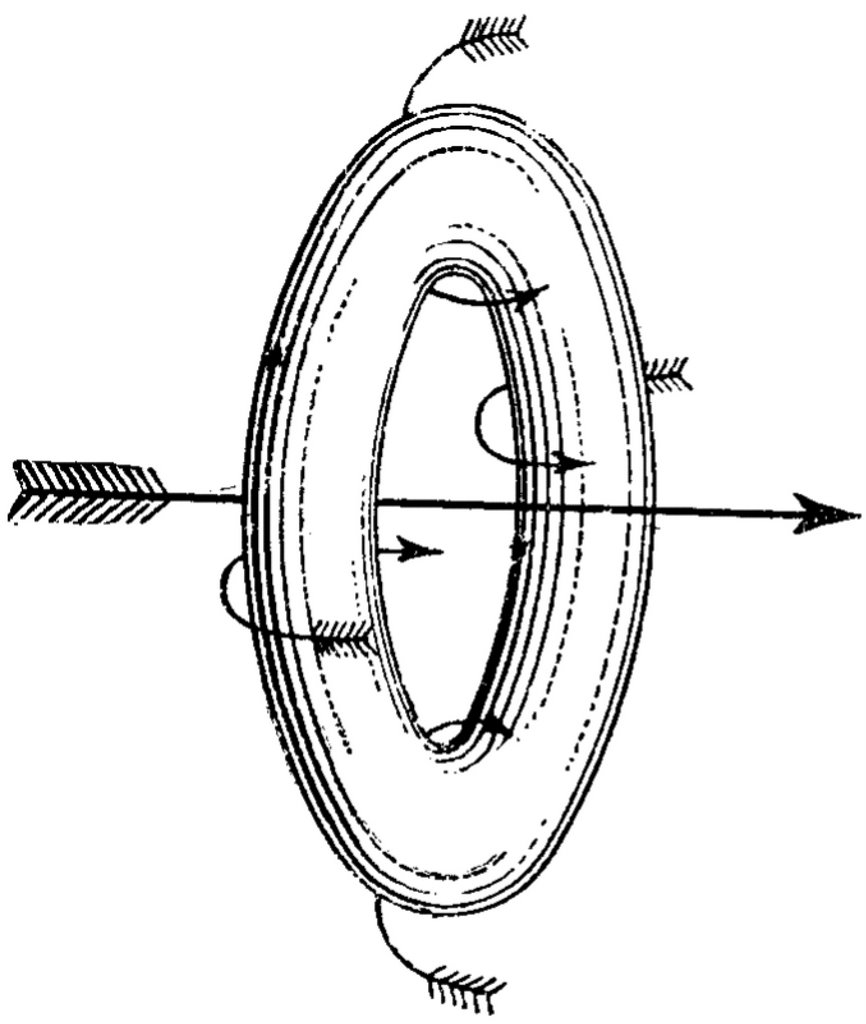
\includegraphics[width=0.7\linewidth]{vortex_titlepage.jpg}
     \caption{\cite{Helmholtz1858}}
     \label{fig:my_label}
 \end{figure}
\newpage
\section*{Abstract}
% Table of contents here
\newpage
\section*{Nomenclature}
\begin{table}[ht]
\begin{tabular}{ll}
Roman and Greek &             \\
$a$             & core radius \\
$\Gamma$        & Vortex circulation   \\
$\rho$             & density   \\
$K$             & Kinetic Energy   \\
$V$             & Self-induced vortex ring velocity \\
$P$             & Impulse
\end{tabular}
\end{table}
\newpage
\section{Introduction}
 Drones pose an ever growing threat to the public whether through accident or malicious intents. When the project was initially set up, there had been isolated cases of near misses between drones and planes and a particular case was discussed when a drone disrupted flights at Gatwick in July 2017 for about 14 minutes \cite{RefWorks:42}. Fast forward to today and everyone's heard of the drones that managed to shut down an airport for approximately $36$ hours and causing about a $1,000$ cancellations and coincidentally the airport was again Gatwick \cite{Gatwick}. No one can dispute that drones pose a serious threat to airports most of whom are inadequately prepared for situations like this. In this instance Gatwick had committed to spending £5 million in anti-drone technology.
\vspace{\baselineskip}

\noindent One possible method we're exploring is using vortex rings to shoot down these drones at airports.
\section{Achievements}
\begin{equation}
    V = \frac{\Gamma}{4\pi R} \left( \ln{\frac{8R}{a} - \alpha}\right)
\end{equation}

\vspace{\baselineskip}
\begin{equation}
    E = \frac{1}{2} \rho R \Gamma^{2}\bigg[\ln{\frac{8}{\epsilon}} - \frac{7}{4} + \frac{3}{16} \epsilon^{2} \ln{\frac{8}{\epsilon}} \bigg]
\end{equation}
Where $\Gamma$ is the circulation and $a$ is the core radius.\cite{dynamics_thin_vortexrings}
\textcolor{red}{TODO: reference equation maybe?}
\newpage
\bibliographystyle{unsrt}
\bibliography{export.bib}
\end{document}